\documentclass{article}

\usepackage[utf8x]{inputenc}
\usepackage[T1]{fontenc}
\usepackage[francais]{babel}
\usepackage{lmodern}
\usepackage{amsthm}
\usepackage{amsmath}
\usepackage{amssymb}
\usepackage{mathrsfs}
\usepackage{verbatim}
\usepackage{moreverb}
\usepackage[top=3cm, bottom=2cm, left=3cm, right=3cm]{geometry}
\usepackage{listings}
\usepackage{graphicx}
\usepackage{hyperref}


\newcommand{\Inde}{\perp \! \! \! \perp}

\lstset{
	basicstyle=\normalsize,
	keywordstyle=\color{blue}, 
	breaklines=true,  
	frame=single,
	morekeywords={*,?php}
}


\hypersetup{colorlinks=true, linkcolor=red}

\author{Conrad \bsc{Hillairet} et Alexandre \bsc{Vieira}}
\title{Projet P2 : Systèmes d'exploitation \\ \Large{PHP}}
\date{\today}

\begin{document}
\maketitle

\setcounter{tocdepth}{4}
\tableofcontents
\newpage

\section*{Introduction}
\addcontentsline{toc}{section}{Introduction} 
Le but de ce projet était de nous faire découvrir le langage PHP et d'approcher un peu la gestion d'une base de données. \\
Le PHP est un langage de script libre inventé en 1994, utilisé principalement sur les serveurs HTTP pour créer des sites internet dynamiques. A la base impératif, ce langage intègre également des fonctionnalités tirées des modèles objets, comme nous le verrons dans les implémentations faîtes un peu plus tard. \\
Un autre avantage du PHP est la possibilité qu'offre ce langage d'utiliser une base de données. Ce point n'est pas le plus développé dans ce projet, mais il est clairement utilisé via un autre langage, le SQL.

\bigskip
Les possibilités offertes par ce langage sont donc très nombreuses et permettent de créer un lien direct entre l'utilisateur et le site internet. C'est ce lien que nous avons voulu montrer dans ce projet, en développant principalement trois grands axes :
\begin{enumerate}
	\item Création d'une page affichant différentes annonces stockées dans une base de données
	\item Création d'un formulaire (dont l'accès est protégé par un mot de passe) permettant d'ajouter une annonce dans la base de données
	\item Création d'une page de contact
\end{enumerate}
Ce dossier présentera d'abord plus en détail le fonctionnement du PHP, puis s'attardera un peu plus sur les différentes implémentations que nous avons effectuées. 

\newpage
\section{Présentation du PHP}
Comme nous venons de le dire, le PHP est un langage de script. Cependant, son fonctionnement est un peu plus complexe que ce qu'on peut connaître avec le Bash ou le CSH, où l'interprétation du code se fait directement sur la machine.
Car après tout, on doit tout de même générer une page compréhensible par un navigateur internet ! C'est ce qu'on va expliquer dans une première sous-partie. On s'intéressera ensuite aux quelques spécificités du codage en PHP, avant de s'intéresser aux bases de données.

\subsection{Fonctionnement global du PHP}
Pour bien comprendre la logique qui se cache derrière le PHP, le mieux est encore de l'illustrer par des schémas, et surtout, de faire le parallèle avec le HTML/CSS.\\
En gros, le fonctionnement d'un site classique fonctionne, schématiquement, ainsi : \\
\begin{center}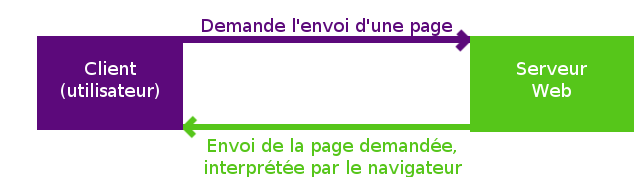
\includegraphics[scale=0.5]{dossier-HTML.png}\end{center}
Dans ce cas, la page renvoyée est en HTML/CSS. C'est le code source, qui est interprété par le navigateur. Il nous affiche alors la page telle qu'il la reçoit, ou plutôt telle qu'il la comprend. Cependant, le navigateur ne peut pas interprété le PHP. Il agit donc au niveau du serveur, ainsi :\\
\begin{center}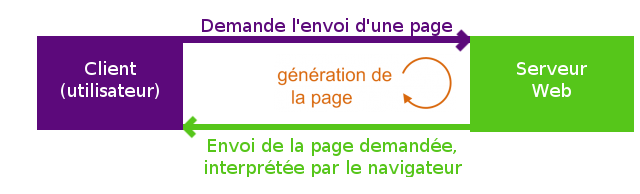
\includegraphics[scale=0.5]{dossier-PHP.png}\end{center}
La page renvoyée est toujours en HTML/CSS, mais elle a été générée par le serveur auparavant. Cela permet donc de faire des pages dynamiques, qui peuvent être modifiées en fonction de nombreux paramètres !\\
Le serveur n'étant rien de plus qu'un gros ordinateur, il peut facilement faire différents calculs, stocker des variables, et surtout les utiliser. La page envoyée au client est donc remodelée à chaque envoi, et le tout est totalement transparent au yeux de l'utilisateur. 

\subsection{A quoi ressemble ce langage ?}
Il faut d'abord voir une chose : le PHP s'utilise en plein milieu de codes HTML. Pour l'utiliser, il faut donc, au préalable, connaître un minimum le langage HTML. \\
Pour différencier le code HTML du code en PHP que le serveur doit interpréter, le code en PHP est placé entre deux balises : \texttt{<?php} et \texttt{?>}.\\
Ces balises peuvent être insérées n'importe où dans le code HTML, et ne seront plus affichées dans le code HTML final, envoyé à l'utilisateur. \\

\bigskip
Ensuite, il faut bien pouvoir dire au serveur ce qu'il doit générer ! On a pour cela, comme dans bien d'autres langages, accès à l'utilisation de variables, l'implémentation de boucles et de conditionnelles, ou encore de fonctions intégrées. \\

\subsubsection{Les variables}
Elles se distinguent très facilement du reste du code par la présence du caractère \$ avant l'identifiant de ces dernières. Comme en bash par exemple, le type des variables n'a pas à être précisé avant d'utiliser la variable, ni même de la déclarer. Le type est déterminé à l'affectation et peut être changé à tout moment. \\
L'affectation se fait d'ailleurs via le signe "=". 

\subsubsection{Les boucles, les conditionnelles}
A ce niveau, les choses ressemblent beaucoup au C. En commençant par les conditionnelles, on a deux syntaxes possibles, qui sont sensiblement les même qu'en C.
\begin{itemize}
	\item \texttt{if...else...} dont la syntaxe est :
		\lstset{language=PHP, keywordstyle=\color{blue}, showstringspaces=false, showtabs=false}  
		\begin{lstlisting}
if (condition1)
	{
		\\Suite d'instructions si condition1 est vraie
	}
elseif (condition2)
	{
		\\Suite d'instructions si condtion1 est fausse et condition2 est vraie
	}
else
	{
		\\Suite d'instructions si condition1 et condition2 sont fausses
	}
		\end{lstlisting}
		Les conditions sont construites de la même façon qu'en C, avec ! pour le NON, \&\& pour le ET, || pour le OU, et ainsi de suite. 

		\bigskip
	\item \texttt{switch} qui permet de construire des conditionnelles plus complexes :
		\begin{lstlisting}
switch(variable)
{
	case valeur1 : //Si variable vaut une certaine valeur
		Instructions;
	case valeur2 :
		Instructions;
	...
	default //Si aucune des conditions ne sont remplies au-dessus
		Instructions;
}
		\end{lstlisting}

\end{itemize}

\bigskip
Les boucles ont une syntaxe qui est également sensiblement la même qu'en C. Elle se font ainsi :
\begin{itemize}
	\item \texttt{while} pour faire une boucle indéterministe :
		\newpage
		\begin{lstlisting}
while (condition)
{
	//Instructions a realiser tant que condition est vrai
}
		\end{lstlisting}

		\bigskip
	\item \texttt{for} pour faire une boucle déterministe :
		\begin{lstlisting}
for ($i=0,$i<$n,$i++)
{
	//Instructions a realiser
}
		\end{lstlisting}
\end{itemize}

\subsubsection{Les fonctions intégrées}
Elles sont très nombreuses, et toutes les lister ici serait superflux. Cependant, on remarque encore une fois un lien très proche avec d'autres langages. En voici quelques exemples :
\begin{itemize}
	\item \texttt{echo} qui permet d'afficher telle quelle une chaîne de caractères ou une variable (qu'on retrouve en bash)
	\item \texttt{strlen} ou \texttt{strtolower} qui renvoie la longueur d'une chaîne dans le premier cas, et qui convertit tous les caractères d'une chaîne en minuscule dans le deuxième cas (qu'on retrouve en C par exemple)
	\item Plusieurs fonctions mathématiques, telles que \texttt{cos} ou \texttt{rand} (qu'on retrouve également en C)
\end{itemize}

\subsection{Les bases de données}
Pour créer des sites dynamiques, les serveurs ont bien souvent besoin d'enregistrer des informations de façon durable. C'est là qu'interviennent les bases de données. On utilise pour cela plusieurs programmes, parmis lesquels :
\begin{itemize}
	\item MySQL
	\item PostgreSQL
	\item Oracle
	\item Et bien d'autres encore
\end{itemize}

Ces programmes s'appellent des SGBD, pour Systèmes de Gestion de Bases de Données. Tous ces SGBD utilisent le même langage pour faire le lien entre le code PHP et la base de données : le SQL. Ce qui change le plus d'un SGBD à l'autre est surtout la manière dont les données seront organisées. 
Dans notre projet, nous avons choisi d'utiliser MySQL.

\bigskip
On peut se demander à quoi sert le PHP dans cette histoire. Il fait en fait le lien entre le développeur et le SGBD. Un schéma valant mieux que de grands mots :\\
\begin{center}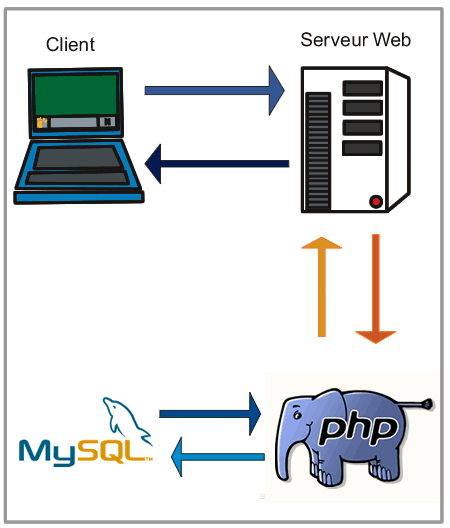
\includegraphics[scale=0.5]{schema2.png}\end{center}
Le serveur, utilisant PHP, interprète le script qui lui est donné. Il rencontre, à un moment, une ligne de SQL. PHP se charge alors de demander à MySQL de traiter l'information. MySQL traite la commande, et renvoie le résultat à PHP, qui se charge de la traiter. 

\bigskip
A présent, voyons comment s'organise une base de données. \\
On distingue trois grandes catégories dans cette organisation :
\begin{itemize}
	\item Il y a tout d'abord \textbf{la base}, qui est la plus haute "boîte" qu'on peut concevoir
	\item Une base est constituée \textbf{d'une ou plusieurs tables}, qui permettent de classer les informations suivant différents critères (le plus souvent, suivant l'utilisation qu'on en fera)
	\item Chaque table est constituée de \textbf{champs} et \textbf{d'entrées}, un peu comme les colonnes et les lignes d'un tableau. 
\end{itemize}

A chaque fois qu'on utilise une base de données, on doit connaître toutes ces informations pour pouvoir correctement l'utiliser. 

\bigskip
On utilise, entre le PHP et le MySQL, différentes fonctions :
\begin{itemize}
	\item On commence par se connecter à la base de données avec la commande suivante : \\
	\begin{center} \texttt{\$bdd = new PDO('mysql:host=NomDeLHost;dbname=NomDeLaBase', 'NomDUtilisateur', 'MotDePasse');} \end{center}
		On reconnaît là le style de la programmation par objet. On crée en effet via cette commande un objet, qui nous permettra par la suite de pouvoir extraire des données de cette base.

		\bigskip
	\item On souhaite, ensuite, récupérer des champs dans une table. On utilise pour cela l'objet précédent :\\
		\begin{center} \texttt{\$reponse = \$bdd -> query(SELECT nomDuChamp1 nomDuChamp2 ... FROM NomDeLaTable WHERE CondtionSurUnChamp)} \end{center}
		On peut remplacer les nomDuChamp par * pour séléctionner tous les champs.\\
		Les commandes comme WHERE forment des critères de séléction. On a, par exemple :
		\begin{itemize}
			\item WHERE permet de séléctionner seulement les champs qui nous intéressent
			\item ORDER BY permet de choisir un champ sur lequel les données seront triées (par ordre alphabétique ou numérique). On rajoute le mot clé DESC si on veut un tri par ordre décroissant
			\item ou encore LIMIT qui permet de limiter le nombre de champ séléctionné
		\end{itemize}

		\bigskip
	\item On récupère enfin les données, entrée par entrée, grâce à l'instruction suivante : 
		\begin{center} \texttt{\$donnees = \$reponse->fetch();} \end{center}
		On utilise souvent cette instruction dans une boucle while, car on récupère les données entrée par entrée, et on peut les afficher ensuite comme on les avait ordonné lors de la récupération des données.

		\bigskip
	\item On veut aussi pouvoir ajouter des données dans la base de données. On utilise pour cela :
	\begin{center} \texttt{\$bdd->exec('INSERT INTO NomTable(NomDesChamps) VALUES(ValeurAAffecterAuxChamps)');} \end{center}
		Cependant, on peut aussi vouloir y rentrer des données variables. On procède pour cela ainsi :
	\begin{center} \texttt{\$req = \$bdd->prepare('INSERT INTO NomTable(NomDesChamps) VALUES(:identifiants)');\\
	\$req->execute(array('identifiant' => \$ValeurVariable,));} \end{center}
	Bien sûr, on doit avoir autant de champs que de valeurs affectées ou d'identifiants, et toujours dans le même ordre pour que l'affectation se fasse bien.

\end{itemize}

\newpage
\section{Présentation de l'implémentation}
Nous avons, dans le cadre de ce projet, réaliser un site web réalisant différentes tâches réalisables en PHP :
\begin{itemize}
	\item Réaliser une page présentant un ensemble de news enregistrées dans une base de données
	\item Créer un formulaire d'ajout de news
	\item Créer un formulaire de contact
\end{itemize}

Le tout est arrangé dans du code HTML pour la mise en page, avec deux feuilles CSS (présentées en Annexe). On inclut également trois pages php qui ne servent qu'à la mise en page, entete.php, menu.php et piedDePage.php, toutes trois également mises en Annexe.
Le résultat est visible sur la page suivante :
\begin{center} \url{http://essaissitesweb.alwaysdata.net/} \end{center}

\subsection{index.php}
Cette page est la première page sur laquelle nous arrivons. Elle présente les news enregistrées dans la base de données, et permet via un formulaire d'accéder au formulaire d'enregistrement de news. Le code est le suivant :
\lstinputlisting[language=HTML]{final/index.php}

\subsection{formul\_news.php}
Via le formulaire de la page précédente, en entrant le bon mot de passe (qui est, sur notre site, MotDePasse), on accède à cette page de formulaire. Elle est très similaire à l'index, mais propose à la place du formulaire d'entrée de mot de passe un formulaire d'entrée de news. Chaque champ rempli est ainsi entré dans la base de données et directement affiché au-dessus.
\lstinputlisting[language=HTML]{final/formul_news.php}

\subsection{enreg\_news.php}
Les données entrées dans la page précédente sont envoyées à ce formulaire qui les traite et les enregistre dans la base de données. On redirige ensuite automatiquement la page vers le formulaire précédent.
\lstinputlisting[language=PHP]{final/enreg_news.php}

\subsection{contact.php}
Cette page propose un formulaire permettant d'envoyer directement un mail à une personne (dont l'adresse est défini dans le script suivant). Cela permet d'automatiser l'envoi de message sans passer par un système de messagerie.
\lstinputlisting[language=HTML]{final/contact.php}

\subsection{envoi\_mail.php}
Ce script php permet de récupérer les données du formulaire précédent et envoi tout cela par mail à une adresse défini dans ce script.
\lstinputlisting[language=PHP]{final/envoi_mail.php}

\newpage
\section*{Conclusion}
\addcontentsline{toc}{section}{Conclusion}
Ce projet nous a permis d'aborder plusieurs points : 
\begin{itemize}
	\item l'apprentissage d'un nouveau langage de programmation, qui rappelle par certains aspects les langages de script et le C
	\item de voir d'une autre manière la programmation par objet et par la même occasion approcher les bases de données
\end{itemize}

\bigskip
Ce projet nous sera sans aucun doute utile dans l'avenir, pour différents petits projets personnels ou même dans le cadre de nos études.

\newpage
\appendix
\section{Bibliographie}
\bsc{Heurtel} Olivier, \textit{PHP5 - Développer un site Web dynamique et intéractif}, Collection Ressouces Informatiques, ENI Editions, 2004

\bigskip
\bsc{Nebra} Mathieu, \textit{Concevez votre site web avec PHP et MySQL }, 2013, disponible \href{http://www.siteduzero.com/informatique/tutoriels/concevez-votre-site-web-avec-php-et-mysql}{ici}

\bigskip
\section{Crédit d'illustration}
Page 6 : schéma trouvé \href{http://www.phpdebutant.org/system/images/intro/schema2.gif}{ici}

\newpage
\section{Annexes}
\subsection{Feuilles CSS}
\lstinputlisting[language=HTML]{final/style.css}
\lstinputlisting[language=HTML]{final/style2.css}

\subsection{entete.php et piedDePage.php}
\lstinputlisting[language=HTML]{final/entete.php}
\lstinputlisting[language=HTML]{final/menu.php}
\lstinputlisting[language=HTML]{final/piedDePage.php}
\end{document}
